\documentclass[twoside]{book}

% Packages required by doxygen
\usepackage{fixltx2e}
\usepackage{calc}
\usepackage{doxygen}
\usepackage[export]{adjustbox} % also loads graphicx
\usepackage{graphicx}
\usepackage[utf8]{inputenc}
\usepackage{makeidx}
\usepackage{multicol}
\usepackage{multirow}
\PassOptionsToPackage{warn}{textcomp}
\usepackage{textcomp}
\usepackage[nointegrals]{wasysym}
\usepackage[table]{xcolor}

% Font selection
\usepackage[T1]{fontenc}
\usepackage[scaled=.90]{helvet}
\usepackage{courier}
\usepackage{amssymb}
\usepackage{sectsty}
\renewcommand{\familydefault}{\sfdefault}
\allsectionsfont{%
  \fontseries{bc}\selectfont%
  \color{darkgray}%
}
\renewcommand{\DoxyLabelFont}{%
  \fontseries{bc}\selectfont%
  \color{darkgray}%
}
\newcommand{\+}{\discretionary{\mbox{\scriptsize$\hookleftarrow$}}{}{}}

% Page & text layout
\usepackage{geometry}
\geometry{%
  a4paper,%
  top=2.5cm,%
  bottom=2.5cm,%
  left=2.5cm,%
  right=2.5cm%
}
\tolerance=750
\hfuzz=15pt
\hbadness=750
\setlength{\emergencystretch}{15pt}
\setlength{\parindent}{0cm}
\setlength{\parskip}{3ex plus 2ex minus 2ex}
\makeatletter
\renewcommand{\paragraph}{%
  \@startsection{paragraph}{4}{0ex}{-1.0ex}{1.0ex}{%
    \normalfont\normalsize\bfseries\SS@parafont%
  }%
}
\renewcommand{\subparagraph}{%
  \@startsection{subparagraph}{5}{0ex}{-1.0ex}{1.0ex}{%
    \normalfont\normalsize\bfseries\SS@subparafont%
  }%
}
\makeatother

% Headers & footers
\usepackage{fancyhdr}
\pagestyle{fancyplain}
\fancyhead[LE]{\fancyplain{}{\bfseries\thepage}}
\fancyhead[CE]{\fancyplain{}{}}
\fancyhead[RE]{\fancyplain{}{\bfseries\leftmark}}
\fancyhead[LO]{\fancyplain{}{\bfseries\rightmark}}
\fancyhead[CO]{\fancyplain{}{}}
\fancyhead[RO]{\fancyplain{}{\bfseries\thepage}}
\fancyfoot[LE]{\fancyplain{}{}}
\fancyfoot[CE]{\fancyplain{}{}}
\fancyfoot[RE]{\fancyplain{}{\bfseries\scriptsize Generated by Doxygen }}
\fancyfoot[LO]{\fancyplain{}{\bfseries\scriptsize Generated by Doxygen }}
\fancyfoot[CO]{\fancyplain{}{}}
\fancyfoot[RO]{\fancyplain{}{}}
\renewcommand{\footrulewidth}{0.4pt}
\renewcommand{\chaptermark}[1]{%
  \markboth{#1}{}%
}
\renewcommand{\sectionmark}[1]{%
  \markright{\thesection\ #1}%
}

% Indices & bibliography
\usepackage{natbib}
\usepackage[titles]{tocloft}
\setcounter{tocdepth}{3}
\setcounter{secnumdepth}{5}
\makeindex

% Hyperlinks (required, but should be loaded last)
\usepackage{ifpdf}
\ifpdf
  \usepackage[pdftex,pagebackref=true]{hyperref}
\else
  \usepackage[ps2pdf,pagebackref=true]{hyperref}
\fi
\hypersetup{%
  colorlinks=true,%
  linkcolor=blue,%
  citecolor=blue,%
  unicode%
}

% Custom commands
\newcommand{\clearemptydoublepage}{%
  \newpage{\pagestyle{empty}\cleardoublepage}%
}

\usepackage{caption}
\captionsetup{labelsep=space,justification=centering,font={bf},singlelinecheck=off,skip=4pt,position=top}

%===== C O N T E N T S =====

\begin{document}

% Titlepage & ToC
\hypersetup{pageanchor=false,
             bookmarksnumbered=true,
             pdfencoding=unicode
            }
\pagenumbering{alph}
\begin{titlepage}
\vspace*{7cm}
\begin{center}%
{\Large fcontrol }\\
\vspace*{1cm}
{\large Generated by Doxygen 1.8.13}\\
\end{center}
\end{titlepage}
\clearemptydoublepage
\pagenumbering{roman}
\tableofcontents
\clearemptydoublepage
\pagenumbering{arabic}
\hypersetup{pageanchor=true}

%--- Begin generated contents ---
\chapter{Hierarchical Index}
\section{Class Hierarchy}
This inheritance list is sorted roughly, but not completely, alphabetically\+:\begin{DoxyCompactList}
\item \contentsline{section}{Block}{\pageref{classBlock}}{}
\begin{DoxyCompactList}
\item \contentsline{section}{F\+System\+Block}{\pageref{classFSystemBlock}}{}
\item \contentsline{section}{P\+I\+D\+Block}{\pageref{classPIDBlock}}{}
\item \contentsline{section}{State\+Variable\+Block}{\pageref{classStateVariableBlock}}{}
\item \contentsline{section}{System\+Block}{\pageref{classSystemBlock}}{}
\begin{DoxyCompactList}
\item \contentsline{section}{Controller\+Block}{\pageref{classControllerBlock}}{}
\end{DoxyCompactList}
\end{DoxyCompactList}
\item \contentsline{section}{Block\+Diagram}{\pageref{classBlockDiagram}}{}
\item \contentsline{section}{Signal\+Sum}{\pageref{classSignalSum}}{}
\item \contentsline{section}{State\+Variable}{\pageref{classStateVariable}}{}
\item \contentsline{section}{System\+Block\+Chain}{\pageref{classSystemBlockChain}}{}
\item \contentsline{section}{Time\+Signal}{\pageref{classTimeSignal}}{}
\item \contentsline{section}{Transfer\+Function}{\pageref{classTransferFunction}}{}
\end{DoxyCompactList}

\chapter{Class Index}
\section{Class List}
Here are the classes, structs, unions and interfaces with brief descriptions\+:\begin{DoxyCompactList}
\item\contentsline{section}{\hyperlink{classBlock}{Block} }{\pageref{classBlock}}{}
\item\contentsline{section}{\hyperlink{classBlockDiagram}{Block\+Diagram} }{\pageref{classBlockDiagram}}{}
\item\contentsline{section}{\hyperlink{classControllerBlock}{Controller\+Block} }{\pageref{classControllerBlock}}{}
\item\contentsline{section}{\hyperlink{classFSystemBlock}{F\+System\+Block} }{\pageref{classFSystemBlock}}{}
\item\contentsline{section}{\hyperlink{classPIDBlock}{P\+I\+D\+Block} }{\pageref{classPIDBlock}}{}
\item\contentsline{section}{\hyperlink{classSignalSum}{Signal\+Sum} }{\pageref{classSignalSum}}{}
\item\contentsline{section}{\hyperlink{classStateVariable}{State\+Variable} }{\pageref{classStateVariable}}{}
\item\contentsline{section}{\hyperlink{classStateVariableBlock}{State\+Variable\+Block} }{\pageref{classStateVariableBlock}}{}
\item\contentsline{section}{\hyperlink{classSystemBlock}{System\+Block} \\*The \hyperlink{classSystemBlock}{System\+Block} class\+: This class encapsulates a system control block, defined by its transference function G. }{\pageref{classSystemBlock}}{}
\item\contentsline{section}{\hyperlink{classSystemBlockChain}{System\+Block\+Chain} }{\pageref{classSystemBlockChain}}{}
\item\contentsline{section}{\hyperlink{classTimeSignal}{Time\+Signal} }{\pageref{classTimeSignal}}{}
\item\contentsline{section}{\hyperlink{classTransferFunction}{Transfer\+Function} }{\pageref{classTransferFunction}}{}
\end{DoxyCompactList}

\chapter{Class Documentation}
\hypertarget{classBlock}{}\section{Block Class Reference}
\label{classBlock}\index{Block@{Block}}


Inheritance diagram for Block\+:\nopagebreak
\begin{figure}[H]
\begin{center}
\leavevmode
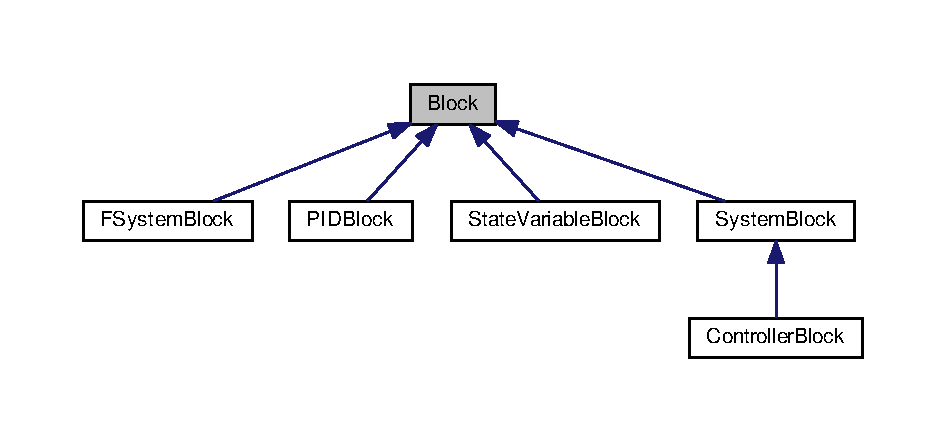
\includegraphics[width=350pt]{classBlock__inherit__graph}
\end{center}
\end{figure}
\subsection*{Public Member Functions}
\begin{DoxyCompactItemize}
\item 
\mbox{\Hypertarget{classBlock_a1a17b39aaed97e601a1b2d508f6034e3}\label{classBlock_a1a17b39aaed97e601a1b2d508f6034e3}} 
long {\bfseries Set\+Saturation} (double low, double high)
\end{DoxyCompactItemize}
\subsection*{Protected Attributes}
\begin{DoxyCompactItemize}
\item 
\mbox{\Hypertarget{classBlock_a9a2c531eb53f86d1c39a819ea7f65935}\label{classBlock_a9a2c531eb53f86d1c39a819ea7f65935}} 
double {\bfseries max\+Out}
\item 
\mbox{\Hypertarget{classBlock_aaad01d77bced26bca7611ae8257c73f7}\label{classBlock_aaad01d77bced26bca7611ae8257c73f7}} 
double {\bfseries min\+Out}
\end{DoxyCompactItemize}
\subsection*{Friends}
\begin{DoxyCompactItemize}
\item 
\mbox{\Hypertarget{classBlock_aff6f40255ea5461398bb769f499016fe}\label{classBlock_aff6f40255ea5461398bb769f499016fe}} 
double {\bfseries operator$>$} (double input, \hyperlink{classBlock}{Block} \&output)
\end{DoxyCompactItemize}


The documentation for this class was generated from the following files\+:\begin{DoxyCompactItemize}
\item 
Block.\+h\item 
Block.\+cpp\end{DoxyCompactItemize}

\hypertarget{classBlockDiagram}{}\section{Block\+Diagram Class Reference}
\label{classBlockDiagram}\index{Block\+Diagram@{Block\+Diagram}}
\subsection*{Public Member Functions}
\begin{DoxyCompactItemize}
\item 
\mbox{\Hypertarget{classBlockDiagram_a5cde235c648f21e5b3fb89ef5db98c49}\label{classBlockDiagram_a5cde235c648f21e5b3fb89ef5db98c49}} 
{\bfseries Block\+Diagram} (std\+::vector$<$ \hyperlink{classBlock}{Block} $\ast$$>$ \&new\+\_\+chain)
\end{DoxyCompactItemize}


The documentation for this class was generated from the following files\+:\begin{DoxyCompactItemize}
\item 
Block\+Diagram.\+h\item 
Block\+Diagram.\+cpp\end{DoxyCompactItemize}

\hypertarget{classControllerBlock}{}\section{Controller\+Block Class Reference}
\label{classControllerBlock}\index{Controller\+Block@{Controller\+Block}}


Inheritance diagram for Controller\+Block\+:\nopagebreak
\begin{figure}[H]
\begin{center}
\leavevmode
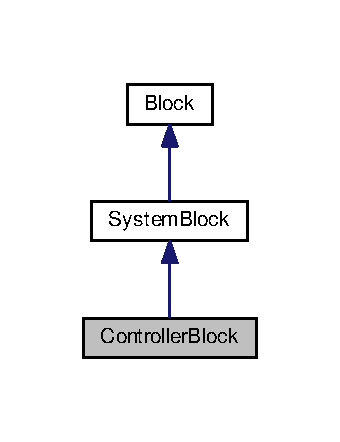
\includegraphics[width=163pt]{classControllerBlock__inherit__graph}
\end{center}
\end{figure}


Collaboration diagram for Controller\+Block\+:\nopagebreak
\begin{figure}[H]
\begin{center}
\leavevmode
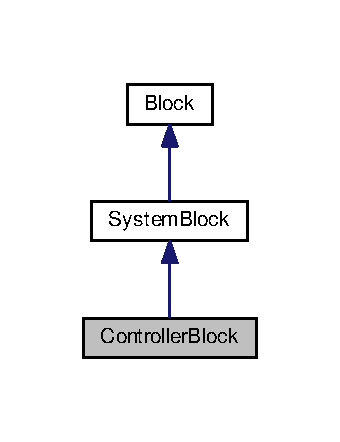
\includegraphics[width=163pt]{classControllerBlock__coll__graph}
\end{center}
\end{figure}
\subsection*{Public Member Functions}
\begin{DoxyCompactItemize}
\item 
\mbox{\Hypertarget{classControllerBlock_a1676a574d7548b7e91b02d8e664a5195}\label{classControllerBlock_a1676a574d7548b7e91b02d8e664a5195}} 
{\bfseries Controller\+Block} (\hyperlink{classTransferFunction}{Transfer\+Function} new\+\_\+transfer)
\item 
\mbox{\Hypertarget{classControllerBlock_ac47b5a7492754f68036a50cd94dee568}\label{classControllerBlock_ac47b5a7492754f68036a50cd94dee568}} 
{\bfseries Controller\+Block} (\hyperlink{classTransferFunction}{Transfer\+Function} new\+\_\+transfer, \hyperlink{classTimeSignal}{Time\+Signal} new\+\_\+signal)
\item 
\mbox{\Hypertarget{classControllerBlock_a06aba555897dacf08e99fdae43683b80}\label{classControllerBlock_a06aba555897dacf08e99fdae43683b80}} 
double {\bfseries Control\+Signal} (double new\+\_\+error)
\end{DoxyCompactItemize}
\subsection*{Additional Inherited Members}


The documentation for this class was generated from the following files\+:\begin{DoxyCompactItemize}
\item 
Controller\+Block.\+h\item 
Controller\+Block.\+cpp\end{DoxyCompactItemize}

\hypertarget{classFSystemBlock}{}\section{F\+System\+Block Class Reference}
\label{classFSystemBlock}\index{F\+System\+Block@{F\+System\+Block}}


Inheritance diagram for F\+System\+Block\+:\nopagebreak
\begin{figure}[H]
\begin{center}
\leavevmode
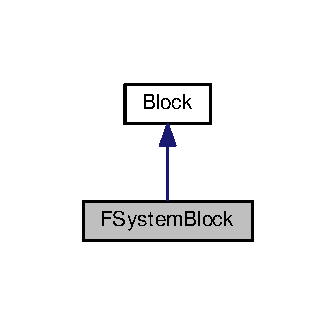
\includegraphics[width=161pt]{classFSystemBlock__inherit__graph}
\end{center}
\end{figure}


Collaboration diagram for F\+System\+Block\+:\nopagebreak
\begin{figure}[H]
\begin{center}
\leavevmode
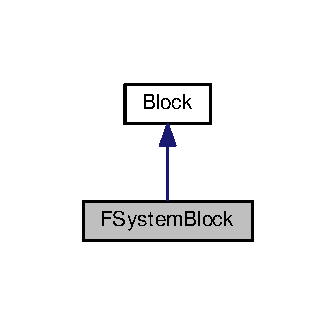
\includegraphics[width=161pt]{classFSystemBlock__coll__graph}
\end{center}
\end{figure}
\subsection*{Public Member Functions}
\begin{DoxyCompactItemize}
\item 
\mbox{\Hypertarget{classFSystemBlock_afeefa2c3dad2736a3a43b132d1a7954f}\label{classFSystemBlock_afeefa2c3dad2736a3a43b132d1a7954f}} 
{\bfseries F\+System\+Block} (const \hyperlink{classTimeSignal}{Time\+Signal} \&time\+Impulse\+Response)
\item 
\mbox{\Hypertarget{classFSystemBlock_aa5bcc98b35e5949b49c7be29a8fdd9bc}\label{classFSystemBlock_aa5bcc98b35e5949b49c7be29a8fdd9bc}} 
bool {\bfseries Time\+Response} (\hyperlink{classTimeSignal}{Time\+Signal} \&input, \hyperlink{classTimeSignal}{Time\+Signal} \&output)
\item 
\mbox{\Hypertarget{classFSystemBlock_a177247b4cfeb76fe43261f28460a4dba}\label{classFSystemBlock_a177247b4cfeb76fe43261f28460a4dba}} 
double {\bfseries Time\+Response\+Update} (const \hyperlink{classTimeSignal}{Time\+Signal} \&old\+\_\+input, const double \&new\+\_\+value)
\item 
\mbox{\Hypertarget{classFSystemBlock_a5462deb7ce710d22bd604bc9e7930b8e}\label{classFSystemBlock_a5462deb7ce710d22bd604bc9e7930b8e}} 
double {\bfseries Output\+Update} (double new\+\_\+input)
\item 
\mbox{\Hypertarget{classFSystemBlock_a726c5fb11e9429c4fd426b4e49685ada}\label{classFSystemBlock_a726c5fb11e9429c4fd426b4e49685ada}} 
bool {\bfseries Signal\+Params} (const \hyperlink{classTimeSignal}{Time\+Signal} \&new\+\_\+signal\+Params)
\end{DoxyCompactItemize}
\subsection*{Additional Inherited Members}


The documentation for this class was generated from the following files\+:\begin{DoxyCompactItemize}
\item 
F\+System\+Block.\+h\item 
F\+System\+Block.\+cpp\end{DoxyCompactItemize}

\hypertarget{classPIDBlock}{}\section{P\+I\+D\+Block Class Reference}
\label{classPIDBlock}\index{P\+I\+D\+Block@{P\+I\+D\+Block}}


Inheritance diagram for P\+I\+D\+Block\+:\nopagebreak
\begin{figure}[H]
\begin{center}
\leavevmode
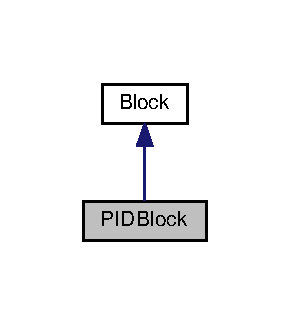
\includegraphics[width=139pt]{classPIDBlock__inherit__graph}
\end{center}
\end{figure}


Collaboration diagram for P\+I\+D\+Block\+:\nopagebreak
\begin{figure}[H]
\begin{center}
\leavevmode
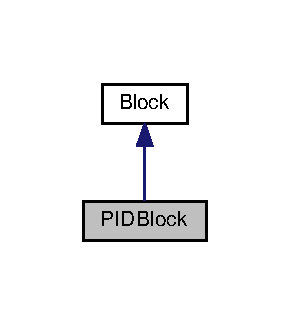
\includegraphics[width=139pt]{classPIDBlock__coll__graph}
\end{center}
\end{figure}
\subsection*{Public Member Functions}
\begin{DoxyCompactItemize}
\item 
\mbox{\Hypertarget{classPIDBlock_a9ec4d61a225f114a32640d2007b35ca8}\label{classPIDBlock_a9ec4d61a225f114a32640d2007b35ca8}} 
{\bfseries P\+I\+D\+Block} (double kp, double ki, double kd, double new\+\_\+\+Ts)
\item 
\mbox{\Hypertarget{classPIDBlock_a69d4c97d0b72eb2d650b5973b3a70073}\label{classPIDBlock_a69d4c97d0b72eb2d650b5973b3a70073}} 
double {\bfseries Update\+Control} (double input)
\item 
\mbox{\Hypertarget{classPIDBlock_aa17a548fbbd21bbc5252c0a07a196dc2}\label{classPIDBlock_aa17a548fbbd21bbc5252c0a07a196dc2}} 
double {\bfseries Output\+Update} (double input)
\item 
\mbox{\Hypertarget{classPIDBlock_a88dc6380a6a8ddb92143f269f1af9adc}\label{classPIDBlock_a88dc6380a6a8ddb92143f269f1af9adc}} 
double {\bfseries Get\+State} () const
\end{DoxyCompactItemize}
\subsection*{Friends}
\begin{DoxyCompactItemize}
\item 
\mbox{\Hypertarget{classPIDBlock_a7c21e4973160d2d1521b4a3095b8e87a}\label{classPIDBlock_a7c21e4973160d2d1521b4a3095b8e87a}} 
double {\bfseries operator$>$} (double input, \hyperlink{classPIDBlock}{P\+I\+D\+Block} \&output)
\end{DoxyCompactItemize}
\subsection*{Additional Inherited Members}


The documentation for this class was generated from the following files\+:\begin{DoxyCompactItemize}
\item 
P\+I\+D\+Block.\+h\item 
P\+I\+D\+Block.\+cpp\end{DoxyCompactItemize}

\hypertarget{classSignalSum}{}\section{Signal\+Sum Class Reference}
\label{classSignalSum}\index{Signal\+Sum@{Signal\+Sum}}


The documentation for this class was generated from the following files\+:\begin{DoxyCompactItemize}
\item 
Signal\+Sum.\+h\item 
Signal\+Sum.\+cpp\end{DoxyCompactItemize}

\hypertarget{classStateVariable}{}\section{State\+Variable Class Reference}
\label{classStateVariable}\index{State\+Variable@{State\+Variable}}
\subsection*{Public Member Functions}
\begin{DoxyCompactItemize}
\item 
\mbox{\Hypertarget{classStateVariable_a7ef7b4dc969e227b1e12930194e6b5fe}\label{classStateVariable_a7ef7b4dc969e227b1e12930194e6b5fe}} 
{\bfseries State\+Variable} (std\+::vector$<$ double $>$ former\+State, std\+::vector$<$ double $>$ initial\+State)
\item 
\mbox{\Hypertarget{classStateVariable_a300c97c1424f1e0478dd937d6249f297}\label{classStateVariable_a300c97c1424f1e0478dd937d6249f297}} 
{\bfseries State\+Variable} (double new\+Value, double D1, double D2)
\item 
\mbox{\Hypertarget{classStateVariable_af7cd47c400edd24b4511850f52106eb3}\label{classStateVariable_af7cd47c400edd24b4511850f52106eb3}} 
long {\bfseries Update} (double new\+Value, double dt)
\item 
\mbox{\Hypertarget{classStateVariable_a33a3fb44ef5d342969646fa8384d3b4d}\label{classStateVariable_a33a3fb44ef5d342969646fa8384d3b4d}} 
double {\bfseries Get\+Order} ()
\item 
\mbox{\Hypertarget{classStateVariable_ad737957a2d383797dae8e693db13307f}\label{classStateVariable_ad737957a2d383797dae8e693db13307f}} 
double {\bfseries D} (uint d\+Order)
\item 
\mbox{\Hypertarget{classStateVariable_a12151f30b145f1301bda0e03952f5d4b}\label{classStateVariable_a12151f30b145f1301bda0e03952f5d4b}} 
std\+::vector$<$ double $>$ {\bfseries get\+State} () const
\item 
\mbox{\Hypertarget{classStateVariable_a2b5b85129f539b4d819977c8da45ba63}\label{classStateVariable_a2b5b85129f539b4d819977c8da45ba63}} 
std\+::vector$<$ double $>$ {\bfseries get\+Former} () const
\end{DoxyCompactItemize}


The documentation for this class was generated from the following files\+:\begin{DoxyCompactItemize}
\item 
State\+Variable.\+h\item 
State\+Variable.\+cpp\end{DoxyCompactItemize}

\hypertarget{classStateVariableBlock}{}\section{State\+Variable\+Block Class Reference}
\label{classStateVariableBlock}\index{State\+Variable\+Block@{State\+Variable\+Block}}


Inheritance diagram for State\+Variable\+Block\+:
\nopagebreak
\begin{figure}[H]
\begin{center}
\leavevmode
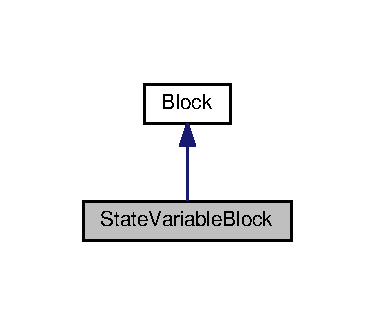
\includegraphics[width=180pt]{classStateVariableBlock__inherit__graph}
\end{center}
\end{figure}


Collaboration diagram for State\+Variable\+Block\+:
\nopagebreak
\begin{figure}[H]
\begin{center}
\leavevmode
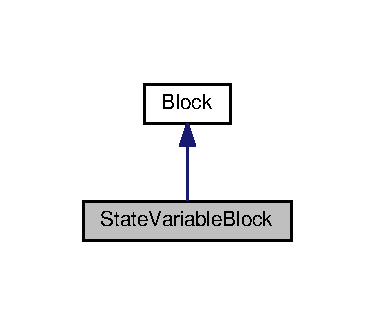
\includegraphics[width=180pt]{classStateVariableBlock__coll__graph}
\end{center}
\end{figure}
\subsection*{Public Member Functions}
\begin{DoxyCompactItemize}
\item 
\mbox{\Hypertarget{classStateVariableBlock_a11e0cfeb7ab94b63a8a5d82d5d41cfc9}\label{classStateVariableBlock_a11e0cfeb7ab94b63a8a5d82d5d41cfc9}} 
{\bfseries State\+Variable\+Block} (double sample\+Time)
\item 
\mbox{\Hypertarget{classStateVariableBlock_a29725438c8df4b7a4ae6822797977a36}\label{classStateVariableBlock_a29725438c8df4b7a4ae6822797977a36}} 
double {\bfseries Output\+Update} (double new\+\_\+input)
\end{DoxyCompactItemize}
\subsection*{Additional Inherited Members}


The documentation for this class was generated from the following files\+:\begin{DoxyCompactItemize}
\item 
State\+Variable\+Block.\+h\item 
State\+Variable\+Block.\+cpp\end{DoxyCompactItemize}

\hypertarget{classSystemBlock}{}\section{System\+Block Class Reference}
\label{classSystemBlock}\index{System\+Block@{System\+Block}}


The \hyperlink{classSystemBlock}{System\+Block} class\+: This class encapsulates a system control block, defined by its transference function G. 




{\ttfamily \#include $<$System\+Block.\+h$>$}



Inheritance diagram for System\+Block\+:\nopagebreak
\begin{figure}[H]
\begin{center}
\leavevmode
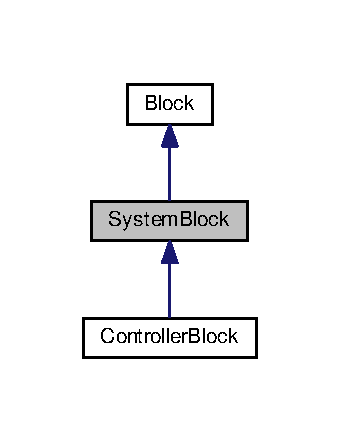
\includegraphics[width=163pt]{classSystemBlock__inherit__graph}
\end{center}
\end{figure}


Collaboration diagram for System\+Block\+:\nopagebreak
\begin{figure}[H]
\begin{center}
\leavevmode
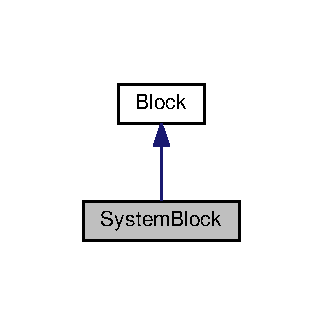
\includegraphics[width=155pt]{classSystemBlock__coll__graph}
\end{center}
\end{figure}
\subsection*{Public Member Functions}
\begin{DoxyCompactItemize}
\item 
\mbox{\Hypertarget{classSystemBlock_a97f55d7953f7a07d8c2290d5039fa5b6}\label{classSystemBlock_a97f55d7953f7a07d8c2290d5039fa5b6}} 
{\bfseries System\+Block} (const std\+::vector$<$ double $>$ \&new\+\_\+num\+Coef, const std\+::vector$<$ double $>$ \&new\+\_\+den\+Coef)
\item 
\mbox{\Hypertarget{classSystemBlock_a2f513f638f6f177b611f8bdd42fc357d}\label{classSystemBlock_a2f513f638f6f177b611f8bdd42fc357d}} 
{\bfseries System\+Block} (const std\+::vector$<$ double $>$ \&new\+\_\+num\+Coef, const std\+::vector$<$ double $>$ \&new\+\_\+den\+Coef, double new\+\_\+gain)
\item 
\mbox{\Hypertarget{classSystemBlock_aebc24f49318e27ce761c34335ee6fe63}\label{classSystemBlock_aebc24f49318e27ce761c34335ee6fe63}} 
{\bfseries System\+Block} (const std\+::vector$<$ double $>$ \&new\+\_\+num\+Coef, const std\+::vector$<$ double $>$ \&new\+\_\+den\+Coef, const std\+::vector$<$ double $>$ \&new\+\_\+num\+Exps, const std\+::vector$<$ double $>$ \&new\+\_\+den\+Exps)
\item 
\mbox{\Hypertarget{classSystemBlock_ac67265b0f826a3fdaf368ba369260c6b}\label{classSystemBlock_ac67265b0f826a3fdaf368ba369260c6b}} 
{\bfseries System\+Block} (const \hyperlink{classTransferFunction}{Transfer\+Function} \&newH)
\item 
\mbox{\Hypertarget{classSystemBlock_a47f1d89600cf61345ca525d90f8d6d6c}\label{classSystemBlock_a47f1d89600cf61345ca525d90f8d6d6c}} 
{\bfseries System\+Block} (double b0, double b1, double a0, double a1)
\item 
\mbox{\Hypertarget{classSystemBlock_a9d9ce9707e97752cb79b7200381fd5eb}\label{classSystemBlock_a9d9ce9707e97752cb79b7200381fd5eb}} 
double {\bfseries Get\+Num\+Order} () const
\item 
\mbox{\Hypertarget{classSystemBlock_aafa63d22e9bc04dfd6785c82fb624c1b}\label{classSystemBlock_aafa63d22e9bc04dfd6785c82fb624c1b}} 
double {\bfseries Get\+Den\+Order} () const
\item 
\mbox{\Hypertarget{classSystemBlock_ac5d4ba30215886e134be5b708d26a85a}\label{classSystemBlock_ac5d4ba30215886e134be5b708d26a85a}} 
long {\bfseries Get\+Transfer} (std\+::vector$<$ double $>$ \&num\+Coefficients, std\+::vector$<$ double $>$ \&den\+Coefficients) const
\item 
\mbox{\Hypertarget{classSystemBlock_ad151469a821fa0ec313d5437cb75a6d6}\label{classSystemBlock_ad151469a821fa0ec313d5437cb75a6d6}} 
virtual double {\bfseries Get\+State} ()
\item 
\mbox{\Hypertarget{classSystemBlock_a2f74c572b6a9527b6b5bde03ba8ab9e6}\label{classSystemBlock_a2f74c572b6a9527b6b5bde03ba8ab9e6}} 
double {\bfseries Output\+Update} (double new\+\_\+input)
\item 
\mbox{\Hypertarget{classSystemBlock_a6162ac92f0d85ff36bff5210cb220871}\label{classSystemBlock_a6162ac92f0d85ff36bff5210cb220871}} 
long {\bfseries Reset} ()
\end{DoxyCompactItemize}
\subsection*{Additional Inherited Members}


\subsection{Detailed Description}
The \hyperlink{classSystemBlock}{System\+Block} class\+: This class encapsulates a system control block, defined by its transference function G.

The documentation for this class was generated from the following files\+:\begin{DoxyCompactItemize}
\item 
System\+Block.\+h\item 
System\+Block.\+cpp\end{DoxyCompactItemize}

\hypertarget{classSystemBlockChain}{}\section{System\+Block\+Chain Class Reference}
\label{classSystemBlockChain}\index{System\+Block\+Chain@{System\+Block\+Chain}}
\subsection*{Public Member Functions}
\begin{DoxyCompactItemize}
\item 
\mbox{\Hypertarget{classSystemBlockChain_a55512b16ad12692b8cf19b7998264dc5}\label{classSystemBlockChain_a55512b16ad12692b8cf19b7998264dc5}} 
{\bfseries System\+Block\+Chain} (const std\+::vector$<$ \hyperlink{classSystemBlock}{System\+Block} $>$ \&new\+\_\+chain)
\item 
\mbox{\Hypertarget{classSystemBlockChain_a1862e5e9f5080db8f37ea5c1c65cd6dd}\label{classSystemBlockChain_a1862e5e9f5080db8f37ea5c1c65cd6dd}} 
bool {\bfseries Time\+Response} (double fs, const std\+::vector$<$ double $>$ \&input, std\+::vector$<$ double $>$ \&output)
\end{DoxyCompactItemize}


The documentation for this class was generated from the following files\+:\begin{DoxyCompactItemize}
\item 
System\+Block\+Chain.\+h\item 
System\+Block\+Chain.\+cpp\end{DoxyCompactItemize}

\hypertarget{classTimeSignal}{}\section{Time\+Signal Class Reference}
\label{classTimeSignal}\index{Time\+Signal@{Time\+Signal}}
\subsection*{Public Member Functions}
\begin{DoxyCompactItemize}
\item 
\mbox{\Hypertarget{classTimeSignal_a18c73bd0180e6b9241285c3227af56a3}\label{classTimeSignal_a18c73bd0180e6b9241285c3227af56a3}} 
{\bfseries Time\+Signal} (unsigned int init\+\_\+size, double init\+\_\+fs)
\item 
\mbox{\Hypertarget{classTimeSignal_ae88ab335c2c3dfbb8e07c0590fe5efba}\label{classTimeSignal_ae88ab335c2c3dfbb8e07c0590fe5efba}} 
{\bfseries Time\+Signal} (std\+::vector$<$ double $>$ new\+\_\+data, double new\+\_\+dts)
\item 
\mbox{\Hypertarget{classTimeSignal_a3c2410005a4590869c53d82dbda73865}\label{classTimeSignal_a3c2410005a4590869c53d82dbda73865}} 
{\bfseries Time\+Signal} (std\+::valarray$<$ double $>$ new\+\_\+data, double new\+\_\+dts)
\item 
\mbox{\Hypertarget{classTimeSignal_af49b9ec38759f4beccd2f3ea916c35d4}\label{classTimeSignal_af49b9ec38759f4beccd2f3ea916c35d4}} 
bool {\bfseries Initialize} (unsigned int new\+\_\+size, double new\+\_\+fs)
\item 
\mbox{\Hypertarget{classTimeSignal_af9aaab7eb101e1d9cac1357d7dc1cd53}\label{classTimeSignal_af9aaab7eb101e1d9cac1357d7dc1cd53}} 
bool {\bfseries Get\+Params} (unsigned int \&out\+\_\+size, double \&out\+\_\+fs) const
\item 
\mbox{\Hypertarget{classTimeSignal_af9b98d58fecd651bfa6e16e3bdf07822}\label{classTimeSignal_af9b98d58fecd651bfa6e16e3bdf07822}} 
double {\bfseries get\+Fs} () const
\item 
\mbox{\Hypertarget{classTimeSignal_ac6947c6308ad45b5da56b6f440bb6bc7}\label{classTimeSignal_ac6947c6308ad45b5da56b6f440bb6bc7}} 
double {\bfseries getN} () const
\item 
\mbox{\Hypertarget{classTimeSignal_aed0b0e8d40fc8806e15a18ed04962ef7}\label{classTimeSignal_aed0b0e8d40fc8806e15a18ed04962ef7}} 
double {\bfseries get\+Dts} () const
\end{DoxyCompactItemize}
\subsection*{Public Attributes}
\begin{DoxyCompactItemize}
\item 
\mbox{\Hypertarget{classTimeSignal_a8f98454a1d25f7d01d8bb7314597f2e9}\label{classTimeSignal_a8f98454a1d25f7d01d8bb7314597f2e9}} 
std\+::valarray$<$ double $>$ {\bfseries data}
\end{DoxyCompactItemize}


The documentation for this class was generated from the following files\+:\begin{DoxyCompactItemize}
\item 
Time\+Signal.\+h\item 
Time\+Signal.\+cpp\end{DoxyCompactItemize}

\hypertarget{classTransferFunction}{}\section{Transfer\+Function Class Reference}
\label{classTransferFunction}\index{Transfer\+Function@{Transfer\+Function}}
\subsection*{Public Member Functions}
\begin{DoxyCompactItemize}
\item 
\mbox{\Hypertarget{classTransferFunction_ac9ae0fe51082390d213e27205f16880c}\label{classTransferFunction_ac9ae0fe51082390d213e27205f16880c}} 
{\bfseries Transfer\+Function} (const std\+::vector$<$ double $>$ \&new\+\_\+num, const std\+::vector$<$ double $>$ \&new\+\_\+den)
\item 
\mbox{\Hypertarget{classTransferFunction_ae93bedeefe64d8679d757ef907914fbd}\label{classTransferFunction_ae93bedeefe64d8679d757ef907914fbd}} 
{\bfseries Transfer\+Function} (const std\+::vector$<$ double $>$ \&new\+\_\+num\+Coef, const std\+::vector$<$ double $>$ \&new\+\_\+den\+Coef, const std\+::vector$<$ double $>$ \&new\+\_\+num\+Exps, const std\+::vector$<$ double $>$ \&new\+\_\+den\+Exps)
\item 
\mbox{\Hypertarget{classTransferFunction_a1810e2b51714e9b3aa2e2e6cf08a6b00}\label{classTransferFunction_a1810e2b51714e9b3aa2e2e6cf08a6b00}} 
std\+::vector$<$ double $>$ {\bfseries get\+Num\+Coef} () const
\item 
\mbox{\Hypertarget{classTransferFunction_a1f8928d9fb90420f6d63cef63fc14199}\label{classTransferFunction_a1f8928d9fb90420f6d63cef63fc14199}} 
std\+::vector$<$ double $>$ {\bfseries get\+Den\+Coef} () const
\item 
\mbox{\Hypertarget{classTransferFunction_a49191b0dced44eae9bfef692323f147a}\label{classTransferFunction_a49191b0dced44eae9bfef692323f147a}} 
std\+::vector$<$ double $>$ {\bfseries get\+Num\+Exps} () const
\item 
\mbox{\Hypertarget{classTransferFunction_a8d202226c249d387acf0da7da2b31ecd}\label{classTransferFunction_a8d202226c249d387acf0da7da2b31ecd}} 
std\+::vector$<$ double $>$ {\bfseries get\+Den\+Exps} () const
\end{DoxyCompactItemize}


The documentation for this class was generated from the following files\+:\begin{DoxyCompactItemize}
\item 
Transfer\+Function.\+h\item 
Transfer\+Function.\+cpp\end{DoxyCompactItemize}

%--- End generated contents ---

% Index
\backmatter
\newpage
\phantomsection
\clearemptydoublepage
\addcontentsline{toc}{chapter}{Index}
\printindex

\end{document}
